\documentclass[onecolumn, draftclsnofoot,10pt, compsoc]{IEEEtran}
\usepackage{graphicx}
\usepackage{url}
\usepackage{setspace}

\usepackage{geometry}
\geometry{textheight=9.5in, textwidth=7in}


% 1. Fill in these details
\def \CapstoneTeamName{		    Nitro ChatBot}
\def \CapstoneTeamNumber{		63}
\def \GroupMemberOne{			Jack Barnes}
\def \GroupMemberTwo{			Sarun Pitaksuteephong}
\def \GroupMemberThree{			Cheng Xie}
\def \CapstoneProjectName{		ChatBot for Load Balancer Infrastructure}
\def \CapstoneSponsorCompany{	OSU Information Services}
\def \CapstoneSponsorPerson{	Stacy Brock}

% 2. Uncomment the appropriate line below so that the document type works
\def \DocType{	%Problem Statement
				Requirements Document
				%Technology Review
				%Design Document
				%Progress Report
				}
			
\newcommand{\NameSigPair}[1]{\par
\makebox[2.75in][r]{#1} \hfil 	\makebox[3.25in]{\makebox[2.25in]{\hrulefill} \hfill		\makebox[.75in]{\hrulefill}}
\par\vspace{-12pt} \textit{\tiny\noindent
\makebox[2.75in]{} \hfil		\makebox[3.25in]{\makebox[2.25in][r]{Signature} \hfill	\makebox[.75in][r]{Date}}}}
% 3. If the document is not to be signed, uncomment the RENEWcommand below
\renewcommand{\NameSigPair}[1]{#1}

%%%%%%%%%%%%%%%%%%%%%%%%%%%%%%%%%%%%%%%
\begin{document}
\begin{titlepage}
    \pagenumbering{gobble}
    \begin{singlespace}
    	%\includegraphics[height=4cm]{logofilename}
        \hfill 
        % 4. If you have a logo, use this includegraphics command to put it on the coversheet.
        %\includegraphics[height=4cm]{CompanyLogo}   
        \par\vspace{.2in}
        \centering
        \scshape{
            \huge CS Capstone \DocType \par
            {\large\today}\par
            \vspace{.5in}
            \textbf{\Huge\CapstoneProjectName}\par
            \vfill
            {\large Prepared for}\par
            \Huge \CapstoneSponsorCompany\par
            \vspace{5pt}
            {\Large\NameSigPair{\CapstoneSponsorPerson}\par}
            {\large Prepared by }\par
            Group\CapstoneTeamNumber\par
            % 5. comment out the line below this one if you do not wish to name your team
            \CapstoneTeamName\par 
            \vspace{5pt}
            {\Large
                \NameSigPair{\GroupMemberOne}\par
                \NameSigPair{\GroupMemberTwo}\par
                \NameSigPair{\GroupMemberThree}\par
            }
            \vspace{20pt}
        }
        \begin{abstract}
        % 6. Fill in your abstract
            This document is an SRS (Software Requirement Specification) which outlines the client requirements for the proposed chatbot software.
            The chatbot will enable users to directly query the status, and modify configurations, for their load balanced resources.
            The requirements within this document serve as a contract with the client and will be used to judge the quality and completeness of the software upon it's 1.0 release.
        \end{abstract}     
    \end{singlespace}
\end{titlepage}
\newpage
\pagenumbering{arabic}
\tableofcontents
% 7. uncomment this (if applicable). Consider adding a page break.
\listoffigures
\listoftables
\clearpage

\textbf{Change History}\par

\begin{tabular}{ p{1in} p{1in} p{4in} }
 \textbf{Revision} & \textbf{Date} & \textbf{Changes} \\
 \hline
 1.0 & 10/26/2019 
 & First Draft \\
 \hline
 1.1 & 11/25/2019 
 & Added language to require direct messages for user commands. Modified language to allow for an additional authentication step. Added mention of a 60 second command response time limit.\\
 \hline
 1.2 & 12/03/2019
 & Fixed broken symbol. Correct spelling error. Created table for user commands. Updated both figures.
\end{tabular}

\clearpage

% 8. now you write!
\section{Introduction}
\subsection{Purpose}
 The software will provide a chatbot interface for users to query the status of their load balanced resources within the Oregon State University network.
 Users with the correct permissions will be able to quickly access the status and perform common configuration tasks on the University's load balancer.
 
\subsection{Scope}
Two primary software components will need to be developed.
The first is the chatbot that will accept commands from a user.
The second software will act as the internal relay, receiving requests from the chatbot, sending commands to the load balancer and then returning the results.
The relay will maintain authentication for active users and perform the direct interaction with the load balancer API (Application Program Interface).
This will allow the chatbot to provide quick access to the status and configuration options for the server pools that the users manage.

\subsection{Product overview}

\subsubsection{Product perspective}
Chatbots are typically used in dialog systems for various practical purposes including customer service or information acquisition \cite{chatbot}.
This proposed implementation of the chatbot exists on top of an existing system and is meant to provide convenient access for the target users.
The chatbot itself will operate as the user interface for users to direct message.
The internal relay will operate as a software interface with the Citrix NetScaler, using it's REST API \cite{citrixnitro}.
\begin{figure}[h]
    \centering
    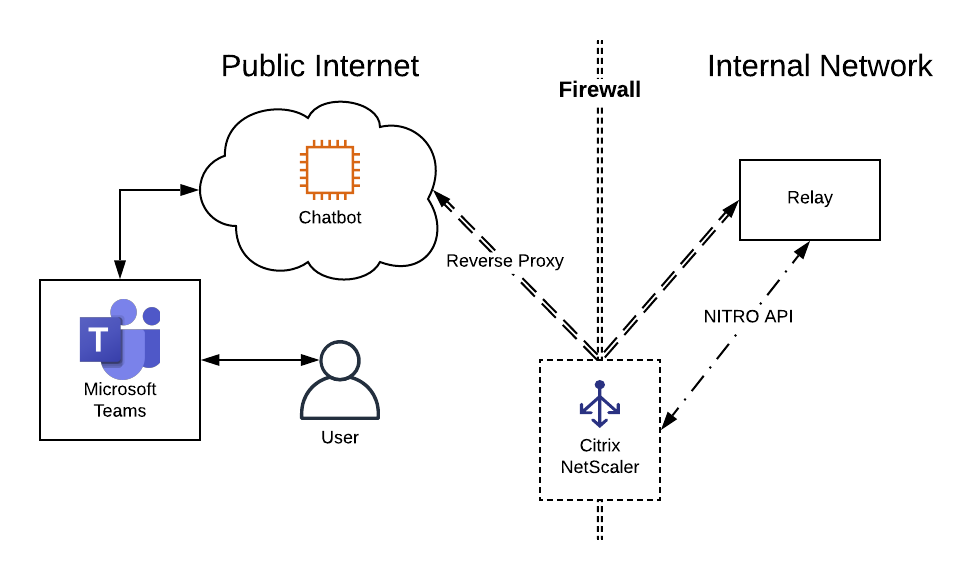
\includegraphics[height=6cm]{overview.png}
    \caption[Basic overview of the chatbot]{Basic overview of the chatbot, and how it will allow users access to load balancer configurations}
    \label{fig:NetScaler Chatbot}
\end{figure}

\subsubsection{Product functions}
The software will have the following major functions:
\\1. The chatbot will begin listening for instruction from a user when it's directly referenced by name.
\\2. The chatbot will accept input from the user and parse input for commands.
\\3. Upon parsing a command, it will securely transmit command and user information to the internal relay.
\\4. The relay will manage authentication
\\5. The relay will send requests to the load balancer through NITRO API
\\6. The relay will transmit results back to the chatbot.
\\7. The chatbot will respond appropriately to user commands.
\\8. The user will not have to authenticate separately outside of Microsoft Teams.
\\9. Users will be able to query for the status of their server pools (including which servers are enabled and disabled).
\\10. Users will be able to query for the status of individual servers.
\\11. Users will be able to enable or disable servers within a pool.
\\12. Users will be able to update certificates for their pools.

\subsubsection{User characteristics}
Users of this chatbot will be system administrators who manage pools of servers at Oregon State University. They have ONID (OSU Network ID) accounts. They have a high-level of technical understanding and are familiar with command line interfaces. The targeted user base is approximately 2 dozen people.
\subsubsection{Limitations}
The chatbot will operate on a common platform accessible to all targeted users.
It will leverage the university's federated login system to identify and properly verify authentication and permissions.
The chatbot must be written in a framework that ensures future portability.
The chatbot itself must be stateless, and not requiring persistent storage.
The chatbot should be (virtually) always available, running on a cloud service within public internet.
A system of CI/CD (Continuous Integration / Continuous Deployment) must also be developed to maintain availability.

\subsection{Definitions}
\underline{Botkit Framework}: An open-source developer tool for building chatbot that also allows custom integration for major messaging platforms. Has direct access to platform APIs. It is owned by Microsoft \cite{framework}.
\\\underline{Chatbot}: A chatbot is a piece of software that conducts a conversation via auditory or textual methods \cite{chatbot}.
\\\underline{Citrix NetScaler}: A an application delivery controller made by Citrix that load balances to make sure that applications can be run as smooth as possible \cite{netscaler}.
\\\underline{Duo}: It is a vendor for cloud-based two-factor authentication service. It can be integrated with any website, VPN (Virtual Private Network), and cloud services \cite{duo}.
\\\underline{Load Balancer}: Load balancer is a reverse proxy that distributes network or application traffic across the server pool. This will increase the efficiency, maintainability, and, speed of the server pool. 
\\\underline{NITRO API}: The NetScaler NITRO protocol allows you to configure and monitor the NetScaler appliance programmatically by using Representational State Transfer (REST) interfaces \cite{citrixnitro}.
\\\underline{ONID}: Oregon State University ID used for identification
\\\underline{REST}: Representational State Transfer. It is a software architect style that defines what could be used for creating web services. The main constraint are the client that uses the API and the resources that the API can provide information to \cite{restphd} \cite{rest}.  
\\\underline{Server Pool}: An autonomous region that contains physical servers. It is a simplified unified view where virtual machines are located \cite{pools}.

\section{Requirements}
\subsection{Apportioning of requirements}
Two separate pieces of software will be defined in these requirements.
This first is referred to as the chatbot, and the second piece of software is referred to as the relay.
These separate pieces of software will be developed separately, but concurrently.
Both have features that rely on the operation of the other.

To assist with development, tests will be written to simulate interaction between the component software.
Features and requirements that span both the chatbot and the relay may be implemented in this fashion at first.
However the feature will not be considered fully implemented until both component software operate with each other.

\subsection{Specified requirements}
The first component software is the chatbot.
The chatbot will run from from a cloud service and operate within a chat platform that can be equally accessed by all users.
The chatbot will be triggered to begin processing input when it's messaged directly, and will not operate by idling within a channel and parsing messages.

When a user messages the chatbot, it will begin parsing input given to it in a manner consistent with command line interfaces.
If the input is invalid, it will tell the user.
If the input in valid, it will initiate communication with the second component software, the relay.
The chatbot will send a request to the relay containing all the necessary information to complete the request, including user information.

When the relay receives a request, it will use the user information to request authentication from the NetScaler.
The relay will communicate requests to the NetScaler using it's REST API, NITRO API.
The relay will maintain and manage authentication in a manner that meets the software requirements.
The relay may require persistent storage to manage and store additional information.

After a user is authenticated, the relay will send the command request to the NetScaler.
Upon receiving a reply from the NetScaler, the relay will format a reply and send it to chatbot.
The chatbot will then format and send the result to the user.
    
\subsection{Functions}
The perspective of the user, the functioning of the software will be quiet simple, with only a small number of commands available.
The intention of the software is to perform these complex configuration tasks as seamlessly as possible.
The chatbot will parse commands from a user when a user directly messages it.
The available functions are detailed below:

\begin{table}[h]
    \caption{Available user commands}
    \begin{tabular}{ p{1.5in} p{2.5in} p{2.5in}  }
     \textbf{Command} & \textbf{Description} & \textbf{Response} \\
     \hline
     status $<$pool-name$>$
     & Query the status of a pool
     & List of servers within the pool and if they are enabled \\
     \hline
     status $<$server-name$>$
     & Query the status of a server
     & The server name and it's current number of active connections \\
     \hline
     enable $<$server-name$>$
     & Enable the server within it's pool
     & Confirmation that the task was completed \\
     \hline
     disable $<$server-name$>$
     & Disable the server within it's pool
     & Confirmation that the task was completed \\
     \hline
     updatecert $<$pool-name$>$
     & Update the certificate for the pool
     & Confirmation that the task was completed \\
     \hline
    \end{tabular}
    \label{tab:commands}
\end{table}

If a user asks to perform a task without proper having permissions, then the bot will respond to the user that they do not have permission to perform the requested task.

\subsection{Performance requirements}
The chatbot is to be, essentially, always available.
It is expected to run continuously on a cloud server, responding to a user when it's messaged directly.
Each user command should be received, processed, and be responded to in a manner of seconds (with 60 seconds being an upper limit).
The chatbot should process commands concurrently, never needing to finish previous requests before new requests are received.
The chatbot should be able to receive command input from multiple sources simultaneously without losing received requests ($<$1\% dropped input). 

\subsection{Usability requirements}
For the user, sending commands through the chatbot should be a seamless experience, minimizing the number of required steps to perform a task.
To achieve this, the chatbot must minimize user interaction while maintaining security.
Initial commands will require an additional authentication step, subsequent commands will use cached information for as long as the authentication token is valid (this depends on implemented protocol).
Given the sensitivity of the user's tasks, security may take precedence over usability when necessary.

The chatbot will accept commands from authorized users in a similar style to command line utilities.
The formatting of the interaction will be first the command, then any applicable flag, followed by additional information.
For example, a user may ask the bot to remove webserver2 from the pool by inputting: "remove webserver2".

\subsection{Interface requirements}
For proper operation and integration of the chatbot and it's relay, both have a number of existing systems that they must interface with.

The chatbot must be deployed to a cloud service to maintain availability. 
This includes designing a system of continuous integration/deployment to allow for remote deployment.
The chatbot must also interface with the chosen chat platform.
Finally, the chatbot must remotely interface with it's relay using a secure connection and common language, through which, it can communicate with the relay.

The relay, the second piece of software, will be deployed internally within the Oregon State University network.
To achieve this, it will likely be deployed as a virtual machine, however the details of this deployment are not statically specified at this time.

The relay must accept a secure connection from the chatbot (which is deployed remotely).
The relay must interpret user information contained within requests from the chatbot to identify and authenticate against the load balancer (Citrix NetScaler).
The relay will interpret commands and send requests to the Citrix NetScaler using it's REST API, NITRO API.

\subsection{Logical database requirements}
Initial software system designs exclude a need for a dedicated database, as the original design is meant to be stateless, without need for persistent storage.
However, the method by which authentication operates may necessitate an external database to match ONID account names to authentication credentials needed to query the NetScaler's API.
Once authenticated, tokens may need to be retained for users that are performing multiple commands in a short amount of time.

\subsection{Design constraints}
The chatbot will be deployed to a cloud service in a manner that allows continuous deployment and continuous integration. 
The relay must utilize the Nitro API to communicate with the NetScaler. 
The chatbot must have a separate relay so that it does not communicate directly with the load balancer.

\subsection{Software system attributes}

\subsubsection{Reliability}
The chatbot or the relay should not crash or produce unspecified states regardless of user input or data received from any interface. 
If the software does halt, or reach an unspecified state, it must be deployed it such a manner that it restarts and restores itself with minimal loss of data or downtime.

\subsubsection{Availability}
The chatbot is intended to be always available.
One exception is the availability of the cloud server/service it's deployed to.
An additional factor in availability, will be the implementation of a messaging system between the chatbot and the relay.
This system must account for connection instability resulting from any number of factors.

\subsubsection{Security}
Security is paramount with the implementation of this software system, as the chatbot will be indirectly communicating with vital network resources.
Users must never be able to request information about, or reconfigure, network resources they don't have explicit permission to modify.

All reconfiguration and status requests must be logged and made accessible to only administrative users.

The relay must interpret requests from the chatbot, never directly passing queries from the chatbot.
The relay must minimize the amount of information that is sent to the chatbot, relaying only what is necessary.

The chatbot should remain stateless, not requiring data persistence during a user's session.
Additionally, the chatbot must never monitor messages that aren't directed at it.

\subsubsection{Portability}
In an attempt to future-proof the chatbot, it will be written using a portable framework.
This will allow the chatbot to be easily portable to different messaging networks, minimizing the work required if an organizational transition occurs.

\clearpage
\section{Appendices}
\subsection{Feature implementation timeline}
\begin{figure}[h]
    \centering
    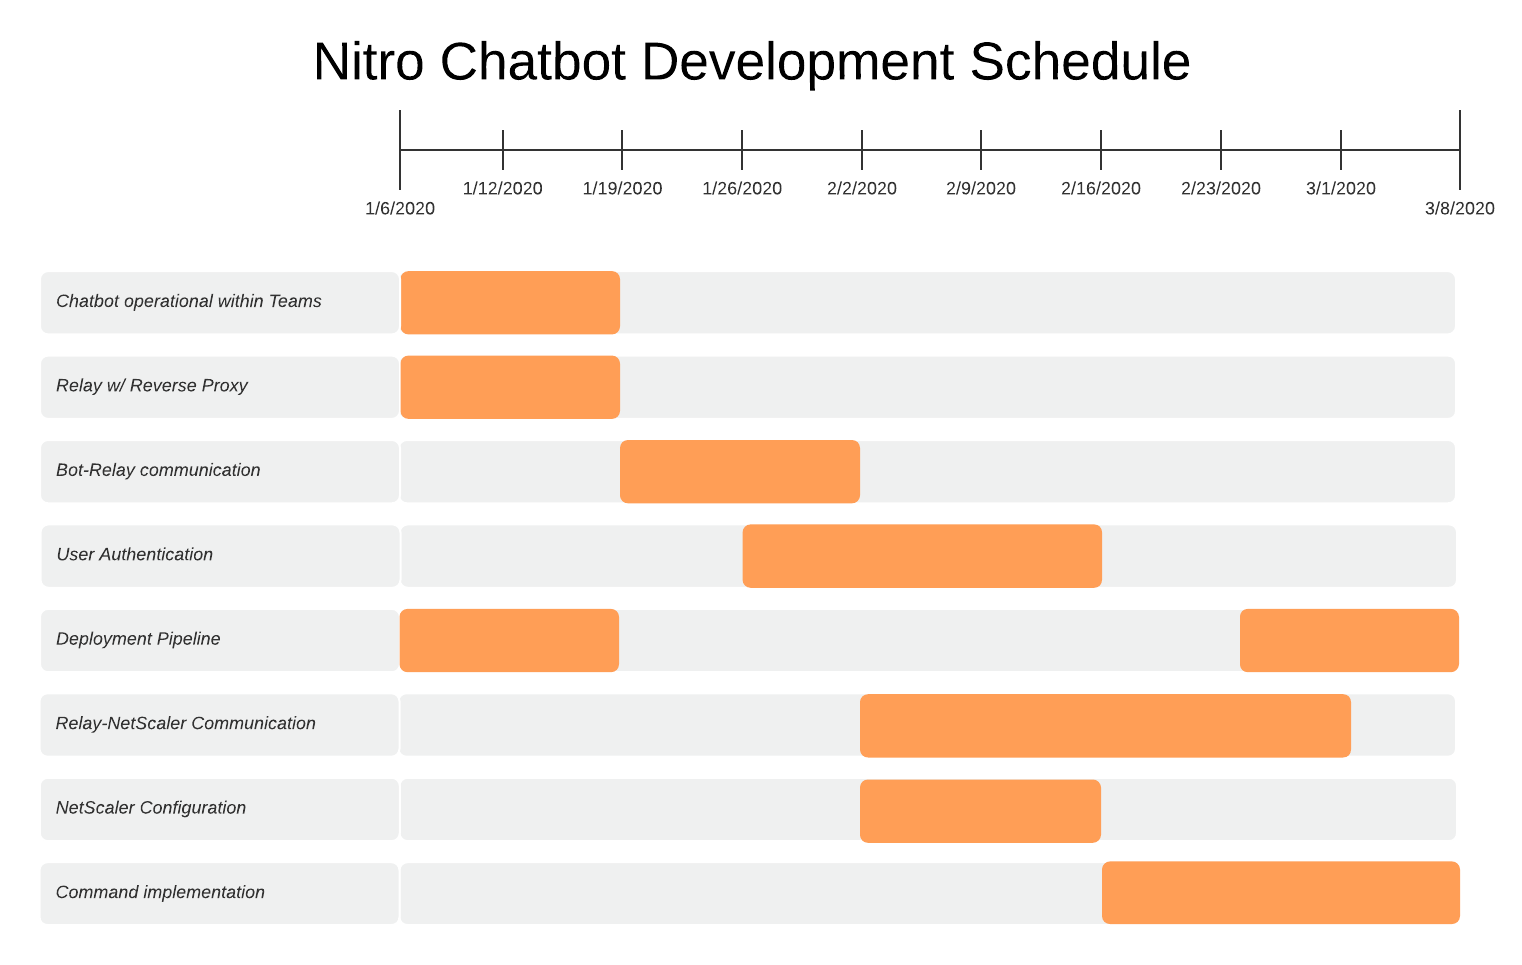
\includegraphics[height=9cm]{gantt.png}
    \caption[Feature implementation timeline]{This is tentative development schedule for Winter term 2020. This timeline give a rough estimation or when features will be implemented.}
    \label{fig:Feature implementation Timeline}
\end{figure}

\clearpage
\bibliographystyle{IEEEtran}
\bibliography{req}

\end{document}
